\documentclass[10pt,twocolumn,twoside]{IEEEtran}


\usepackage{cite}
\usepackage[pdftex]{graphicx}
\usepackage[cmex10]{amsmath}
\usepackage{amsfonts}
\usepackage{algorithmic}
\usepackage{array}
\usepackage{mdwmath}
\usepackage{mdwtab}
\usepackage[caption=false,font=footnotesize]{subfig}
\usepackage{fixltx2e}
\usepackage{url}
\usepackage{color}

\graphicspath{{./images/}{./images/finance/}{./images/tracking/}}
%\interdisplaylinepenalty=1000

\newenvironment{meta}[0]{\color{red} \em}{}

% correct bad hyphenation here
\hyphenation{}

\begin{document}

\title{Particle Smoothing Algorithms for Variable Rate Models}

\author{Pete~Bunch*,~\IEEEmembership{Member,~IEEE,}
        Simon~Godsill,~\IEEEmembership{Member,~IEEE,}% <-this % stops a space
\thanks{P. Bunch and S. Godsill are with the Department
of Engineering, Cambridge University, UK. email: \{pb404,sjg30\}@cam.ac.uk}% <-this % stops a space
}%\thanks{Manuscript received January 01, 1901; revised January 02, 1901.}}


% The paper headers
\markboth{IEEE Transaction in Signal Processing}{IEEE Transaction in Signal Processing}%,~Vol.~1, No.~1, January~1901}%
%{Bunch \& Godsill: Particle Smoothing Algorithms for Variable Rate Models}

% make the title area
\maketitle

\begin{abstract}
Standard state-space methods assume that the latent state evolves uniformly over time, and can be modelled with a discrete-time process synchronous with the observations. This may be a poor representation of some systems in which the state evolution displays discontinuities in its behaviour. For such cases, a variable rate model may be more appropriate; the system dynamics are conditioned on a set of random changepoints which constitute a marked point process. In this paper, new particle smoothing algorithms are presented for use with conditionally linear-Gaussian and conditionally deterministic dynamics. These are demonstrated on problems in financial modelling and target tracking. Results indicate that the smoothing approximations provide more accurate and more diverse representations of the state posterior distributions.
\end{abstract}

\begin{IEEEkeywords}
Bayesian inference, state-space model, variable rate, particle filter, filtering, smoothing
\end{IEEEkeywords}



\section{Introduction}

\IEEEPARstart{T}{he} objective of sequential Bayesian inference is to estimate an imperfectly observed quantity as it varies over time. This is accomplished through the use of probabilistic models for the state evolution and measurement processes. Often, the latent state is a continuously varying quantity, whereas the observations are made at a discrete set of times. In these circumstances, it is simplest to discretise the state onto the same set of times as the observations. When the system is also Markovian, this leads to the standard ``fixed rate'' hidden Markov model (HMM). The standard HMM is poorly suited to systems where the state evolution contains discontinuities; for example, the price of a financial asset which may display large jumps at random times between periods of diffusion-like behaviour, or the kinematic state of a manoeuvring vehicle which may have sudden changes in the acceleration when turns begin or end. Such problems can be handled more naturally using a ``variable rate'' model, in which the state dynamics are conditioned upon a set of changepoints which characterise transitions in behaviour.

In a variable rate setting, changepoints and associated parameters are modelled as a marked point process (MPP), the mathematical properties of which are explored comprehensively in \cite{Jacobsen2006}. Conditional upon this MPP the state evolves according to some benign dynamics. In \cite{Godsill2007,Whiteley2011}, the conditional state evolution is treated as deterministic, while in \cite{Godsill2007a,Christensen2012} a conditionally linear-Gaussian state model is considered.

The posterior distribution for the changepoint MPP is inherently nonlinear, and cannot be calculated analytically. Instead, inference may be conducted using numerical approximations. The particle filter (introduced by \cite{Gordon1993}) and smoother (see \cite{Doucet2000a,Godsill2004}) are schemes which approximate a posterior distribution using a set of samples, or ``particles'', drawn sequentially from it.  A thorough introduction to particle filtering and smoothing methods can be found in \cite{Cappe2007,Doucet2009}. In \cite{Godsill2007a,Godsill2007,Whiteley2011}, the particle filter was adapted for use with variable rate models, resulting in the variable rate particle filter (VRPF).

The VRPF allows the changepoint sequence --- and hence the current state --- to be estimated sequentially as observations are received. However, estimates can often be improved later once further observations have been made. In this paper, we address the problem of smoothing in variable rate models, i.e. the estimation of the changepoint sequence and latent state given all the observations. We achieve this with an efficient backward sweep through the observations, in a new version of the method for standard HMMs described in \cite{Godsill2004}. Two new schemes are introduced: one for conditionally linear-Gaussian models which exploits the method of Rao-Blackwellisation; and a second for use with conditionally-deterministic models which uses an augmented target distribution in the style of an SMC sampler \cite{DelMoral2006}.

We introduce the general structure of variable rate models in section~\ref{sec:vr_models}. The VRPF is reviewed in section~\ref{sec:vrpf}, and new variable rate smoothing algorithms are described in section~\ref{sec:vrps}. In section~\ref{sec:simulations}, algorithm performance is demonstrated through simulations.



\section{Variable Rate Models} \label{sec:vr_models}

We consider a general model from time $0$ to $T$, between which observations, $\{y_1 \dots y_N\}$, are made at times $\{t_1 \dots t_N = T\}$. During this period, an unknown number of changepoints, $K$, occur at times $\{\tau_0 = 0, \tau_1 \dots \tau_K \}$, each with associated changepoint parameters, $\{ u_0, u_1 \dots u_K \}$. The pairs $\{\tau_k, u_k\}$ are the elements of a marked point process (MPP). The latent state is a continuous-time process denoted $x(t)$. Discrete sets containing multiple values over time will be written as, e.g. $y_{1:n} = \{y_1 \dots y_n\}$.

The objective for inference will be to estimate the changepoint sequence. This will be denoted as $\theta = \{\tau_{0:K}, u_{0:K}\}$. At a particular time $t_n$, the sequence will be divided into past $\theta_n^- = \{\tau_{j}, u_{j} \forall j : 0 \leq \tau_j < t_n \}$, and future $\theta_n^+ = \{\tau_{j}, u_{j} \forall j : t_n \leq \tau_j < T \}$. It will also be useful to define a variable for the changepoints which occur in the interval $[t_{n-1},t_n)$, $\theta_{n \setminus n-1} = \{\tau_{j}, u_{j} \forall j : t_{n-1} \leq \tau_j < t_n \}$.

For notational simplicity, the following counting variables are introduced to keep track of the most recent changepoint to have occurred,
%
\begin{IEEEeqnarray}{rCl}
 K(t)  & = & \max(k : \tau_k<t) \\
 K_n   & = & K(t_n)     .
\end{IEEEeqnarray}

The changepoint sequence is assumed to be a Markov process,
%
\begin{IEEEeqnarray}{rCl}
 \{\tau_k, u_k\} & \sim & p(\tau_k, u_k|\tau_{k-1}, u_{k-1}) \label{eq:cp_model}     .
\end{IEEEeqnarray}

This density will be constructed such that $P(\tau_k < \tau_{k-1}) = 0$. As in \cite{Whiteley2011}, a survivor function is defined as the probability that no new changepoint occurs before a given time,
%
\begin{IEEEeqnarray}{rCl}
 S(\tau_k, u_k, t) &=& P(\tau_{k+1}>t|\tau_k, u_k) \nonumber \\
              &=& 1 - \int_{\tau_k}^{t} p(\xi|\tau_{k}, u_k) d\xi     .
\end{IEEEeqnarray}

It is now possible to write down a prior for the changepoint sequence. This comprises a density term for each changepoint in the sequence and a survivor function term accounting for the probability that no additional changepoints occur within the time interval. We use the convention that $\tau_0 = 0$.

\begin{IEEEeqnarray}{rCl}
p(\theta_n^-) & = & S(\tau_{K_n},u_{K_n},t_n) p(u_0) \prod_{k=1}^{K_n} p(\tau_k, u_k| \tau_{k-1}, u_{k-1}) \label{eq:cp_sequence_prior}
\end{IEEEeqnarray}

The existence of such a density for a MPP is addressed in \cite{Jacobsen2006}. The number of changepoints, $K_n$, is not fixed. If $u_k$ varies over $\mathcal{U}$, and $\tau_k$ varies over the real line $\mathbb{R}$, then the space spanned by $\theta_n^-$ is the union,
%
\begin{IEEEeqnarray}{rCl}
 \Theta & = & \bigcup_k \Theta_k \label{eq:theta_space} \\
 \Theta_k & = & \{k\} \times \mathbb{R}^k \times \mathcal{U}^k     .
\end{IEEEeqnarray}

This closely resembles the variable-dimension spaces employed by reversible jump Markov chain Monte Carlo (MCMC) algorithms \cite{Green1995}.% or in multiple target tracking scenarios \cite{Vo2005}.



\subsection{Conditionally Linear-Gaussian Models} \label{sec:clg_models}

We first consider the class of variable rate models whose state dynamics are linear-Gaussian conditional on the changepoint sequence. Such a model may be discretised onto the set of observation times in exactly the same manner as a standard HMM,
%
\begin{IEEEeqnarray}{rCl}
 x_n & = & A_n(\theta_{n}^-)x_{n-1} + w_n \\
 y_n & = & C_n(\theta_{n}^-)x_n + v_n       ,
\end{IEEEeqnarray}

where $w_n$ and $v_n$ are independent Gaussian variables (although the independence condition may be relaxed \cite{Grewal2002}),
%
\begin{IEEEeqnarray}{rCl}
 w_n & \sim & \mathcal{N}(w_n|0, Q_n(\theta_{n}^-)) \\
 v_n & \sim & \mathcal{N}(v_n|0, R_n(\theta_{n}^-))       .
\end{IEEEeqnarray}

In addition, the prior state distribution should be Gaussian, with known mean and covariance,
%
\begin{IEEEeqnarray}{rCl}
 x_0 & \sim & \mathcal{N}(x_0|m_0, P_0)       .
\end{IEEEeqnarray}

If the changepoint sequence is known, or has been estimated, then the state posterior distributions may be inferred conditionally using optimal Kalman filtering and smoothing recursions. As well as the basic Kalman filter \cite{Kalman1960}, the Rauch-Tung-Striebel (RTS) smoother \cite{Rauch1965} and two-filter smoother \cite{Fraser1969} will prove useful for this step later in the paper.



\subsubsection*{A Jump-Diffusion model for Financial Assets} \label{sec:financial_model}

Conditionally linear-Gaussian models for use with variable rate particle filters were introduced in \cite{Godsill2007a,Christensen2012} for financial applications. A version of these models is used for testing the new smoothing algorithm. Prices of an asset are treated as noisy observations of a latent state, which evolves according to a drift-diffusion with occasional jumps.

The state is a vector with two elements, the underlying value of the asset, and the trend followed by this value,
%
\begin{equation}
 x(t) = [ z(t), \dot{z}(t)]^T     .
\end{equation}

This evolves continuously according to a jump-diffusion model,
%
\begin{IEEEeqnarray}{c}
 dx(t) = \begin{bmatrix}0 & 1 \\ 0 & -\lambda \end{bmatrix} x(t) dt + \begin{bmatrix}0 \\ \sigma \end{bmatrix} d\beta(t) + dJ(t)
\end{IEEEeqnarray}

where $\lambda$ introduces a mean reversion effect on the trend and $\beta(t)$ is standard Brownian motion (with unit diffusion constant). The jump term, $dJ(t)$, is zero everywhere except when jumps occur,
%
\begin{IEEEeqnarray}{rCl}
 dJ(t) & = & \begin{cases} J_k & t \in \{\tau_k\} \\ 0 & \text{elsewhere} \end{cases} \\
 J_k  & \sim & \mathcal{N}(J_k| 0, Q_{J,u_k})     .
\end{IEEEeqnarray}

$\{\tau_k\}$ is the set of random jump times, each of which is one of two types: a value jump, indicated by $u_k = 1$, or a trend jump, indicated by $u_k=2$. The jump covariance matrices are,
%
\begin{IEEEeqnarray}{c}
Q_{J,u_k} = \begin{cases} \begin{bmatrix}\sigma_{J1}^2 & 0 \\ 0 & 0 \end{bmatrix} & u_k = 1 \\
                          \begin{bmatrix}0 & 0 \\ 0 & \sigma_{J2}^2 \end{bmatrix} & u_k = 2  \end{cases}   .
\end{IEEEeqnarray}

Only the value is observed, and that corrupted by additive Gaussian noise with standard deviation $\sigma_y^2$.

This model may be discretised at the observation times using standard methods, detailed in appendix~\ref{app:lg_model_discretisation}, leading to,% (see \cite{Godsill2007a,Christensen2012,Grewal2002}), leading to,
%
%Assuming observations of value only and Gaussian observation noise with standard deviation $\sigma_y^2$, the resulting discrete time dynamics are described by the following equations:% (see appendix \ref{app:model_discretisation}):
%
\begin{IEEEeqnarray}{rCl}
 x_n & = & A x_{n-1} + w_n \\
 y_n & = & C x_{n} + v_n
\end{IEEEeqnarray}

where the $w_n$ and $v_n$ are Gaussian random variables with covariance matrixes $Q_n$ and $R$ respectively. $Q_n$ is a function of the sequence of jump times and their types, giving rise to the desired conditionally linear-Gaussian structure.




\subsection{Conditionally Deterministic Models} \label{sec:cd_models}

Next we examine the class of variable rate models in which the state is completely specified by the changepoint sequence, with no additional random components. Such a process is commonly referred to as ``piecewise-deterministic'', as the latent state follows a deterministic path between changepoints. In this case, it is not necessary to discretise the state --- it may be kept as a continuous variable.

In general, the state dynamics will be governed by a differential equation which may depend on the entire changepoint sequence. Here we assume that only the most recent changepoint determines the future state trajectory,
%
\begin{IEEEeqnarray}{rCl}
 dx(t) & = & \varphi(x(t), \tau_{K(t)}, u_{K(t)}) dt     .
\end{IEEEeqnarray}

By introducing a new sequence, $\{ x_0, x_1 \dots x_K \}$, which denotes the value of the state at each changepoint (i.e. $x_k = x(\tau_k)$), and assuming that an analytic solution exists, a piecewise function describing the path may be found,
%
\begin{IEEEeqnarray}{rCll}
 x(t) & = & f(x_{K_n}, u_{K_n}, \tau_{K_n}, t) &, \tau_{K_n} < t \leq \tau_{K_{n}+1}    \label{eq:disc_time_state_diff_eq}     .
\end{IEEEeqnarray}

By choosing $t = \tau_{K_{n}+1}$, this equation specifies the state at the next changepoint time. Similarly, by choosing $t=t_n$, the state at the observation times may be evaluated --- these latter points will be denoted $\hat{x}_n$. To complete the framework, a probabilistic measurement model must be devised for the observation process, $p(y_n|\hat{x}_n)$.

For convenience, we assume that $x_0$ is known in the following sections. This means that $x(t)$ may be calculated deterministically for all $t$ given $\theta$. This condition is easily relaxed by including $x_0$ as a random variable in the posterior distribution.



\subsubsection*{An Intrinsic Coordinate Model for Manoeuvring Vehicles} \label{sec:tracking_model}

Target tracking algorithms are commonly based upon fixed rate models (see, e.g. \cite{Li2003} for a thorough survey), in which the target kinematics (position, velocity, etc.) are estimated at a set of fixed times at which observations (e.g. radar measurements) are made. In \cite{Godsill2007a,Godsill2007,Whiteley2011,Bunch2012a}, variable rate models were introduced for tracking. The state trajectory is divided up by a set of changepoints, between which the motion follows a deterministic path governed by motion parameters (accelerations, etc.) which are fixed for that division. In this paper we use the 2-dimensional intrinsic coordinate model of \cite{Bunch2012a} to test the new smoothing algorithm.

The target is modelled as a particle subject to perpendicular forces tangential and normal to the direction of motion. These forces are held constant between changepoint times, $\tau_{1:K}$, which represent the beginnings and ends of manoeuvres. The state vector consists of Cartesian position, $x_1(t)$ and $x_2(t)$, plus heading angle, $\psi(t)$, and speed, $\dot{s}(t)$,
%
\begin{equation}
x(t) = [x_1(t), x_2(t), \psi(t), \dot{s}(t)]^T     .
\end{equation}

In addition to the tangential and normal accelerations, $a_{T,k}$ and $a_{N,k}$, we introduce two linear velocity terms, $d_{X,k}$ and $d_{Y,k}$. As will become apparent later, these are necessary for the operation of an efficient smoothing algorithm. They provide us with enough degrees of freedom to match the state trajectory between an arbitrary past changepoint ($\tau_{K(t)}$, $\mathbf{x}_{K(t)}$) and an arbitrary future changepoint ($\tau_{K(t)+1}$, $\mathbf{x}_{K(t)+1}$). These linear velocity parameters may be considered to be merely relaxation terms, or they may represent real physical effects, such as wind (for aircraft) or currents (for boats). Together, these four variables make up the vector of motion parameters,
%
\begin{equation}
u_k = [a_{T,k}, a_{N,k}, d_{X,k}, d_{Y,k}]^T     .
\end{equation}

The target dynamics are described by four differential equations,
%
\begin{IEEEeqnarray}{rCl}
\ddot{s}(t) & = & a_{T,K(t)} \\
\dot{s}(t) \dot{\psi}(t) & = & a_{N,K(t)} \\
\dot{x}_{1}(t) & = & \dot{s}(t) \cos(\psi(t)) + d_{X,K(t)} \\
\dot{x}_{2}(t) & = & \dot{s}(t) \sin(\psi(t)) + d_{Y,K(t)}     .
\end{IEEEeqnarray}

Solving these yields the following state equations (where $\Delta\ t = t - \tau_{K(t)}$),
%
\begin{IEEEeqnarray}{rCl}
\dot{s}(t) & = & \dot{s}_{K(t)} + a_{T,k} \Delta t \label{eq:2D_ICmodel_1} \\
\psi(t) & = & \psi_{K(t)} + \frac{a_{N,k}}{a_{T,k}} \log \left( \frac{\dot{s}(t)}{\dot{s}_{K(t)}} \right) \label{eq:2D_ICmodel_2}
\end{IEEEeqnarray}
\begin{IEEEeqnarray}{rCl}
x_1(t) & = & x_{1,K(t)} + d_{X,K(t)} \Delta t \label{eq:2D_ICmodel_3} \\
     \IEEEeqnarraymulticol{3}{l}{ \quad + \: \frac{ \dot{s}(t)^2 }{ 4 a_{T,k}^2 + a_{N,k}^2 } \left[  a_{N,k} \sin(\psi(t)) + 2 a_{T,k} \cos(\psi(t))  \right]} \nonumber \\
     \IEEEeqnarraymulticol{3}{l}{ \quad - \: \frac{\dot{s}_{K(t)}^2}{4 a_{T,k}^2 + a_{N,k}^2} \left[  a_{N,k} \sin(\psi_{K(t)}) + 2 a_{T,k} \cos(\psi_{K(t)})  \right]} \nonumber
\end{IEEEeqnarray}
\begin{IEEEeqnarray}{rCl}
x_2(t) & = & x_{2,K(t)} + d_{Y,K(t)} \Delta t \label{eq:2D_ICmodel_4} \\
     \IEEEeqnarraymulticol{3}{l}{ \quad + \: \frac{ \dot{s}(t)^2 }{ 4 a_{T,k}^2 + a_{N,k}^2 } \left[ -a_{N,k} \cos(\psi(t)) + 2 a_{T,k} \sin(\psi(t))  \right]} \nonumber \\
     \IEEEeqnarraymulticol{3}{l}{ \quad - \: \frac{\dot{s}_{K(t)}^2}{4 a_{T,k}^2 + a_{N,k}^2} \left[  -a_{N,k} \cos(\psi_{K(t)}) + 2 a_{T,k} \sin(\psi_{K(t)})  \right]} \nonumber      .
\end{IEEEeqnarray}

When formulating the smoothing algorithm, it will be necessary that $u_k$ can be calculated for any pair of adjacent changepoints, $(\tau_k,x_k)$, and $(\tau_{k+1},x_{k+1})$. This condition is met by the preceding model --- the equations are solved in the order specified to find $a_{T,k}$ from (\ref{eq:2D_ICmodel_1}), $a_{N,k}$ from (\ref{eq:2D_ICmodel_2}), and finally $d_{X,K(t)}$ and $d_{Y,K(t)}$ from (\ref{eq:2D_ICmodel_3}) and (\ref{eq:2D_ICmodel_4}).



\section{The Variable Rate Particle Filter} \label{sec:vrpf}

The variable rate particle filter (VRPF) is described in \cite{Godsill2007,Godsill2007a,Whiteley2011}. The objective of the algorithm is to sequentially estimate the posterior distribution of the changepoint sequence, $p(\theta_{n}^-| y_{1:n})$, at each time $t_n$, which is defined on the same space as the prior density (\ref{eq:theta_space}). This distribution may be expanded using Bayes' rule,
%
\begin{IEEEeqnarray}{rCl}
\IEEEeqnarraymulticol{3}{l}{ p(\theta_{n}^-|y_{1:n}) \propto p(y_n|\theta_{n}^-, y_{1:n-1}) } \nonumber \\
 \qquad & & \times p(\theta_{n \setminus n-1}|\theta_{n-1}^-) p(\theta_{n-1}^-|y_{1:n-1}) \label{eq:vrpf_target}     .
\end{IEEEeqnarray}

The transition term, $p(\theta_{n \setminus n-1} | \theta_{n-1}^-)$, has a similar form to the changepoint prior of (\ref{eq:cp_sequence_prior}) \cite{Jacobsen2006}, but an additional survivor function is included to account for the condition that changepoints cannot occur before $t_{n-1}$,
%
\begin{IEEEeqnarray}{rCl}
\IEEEeqnarraymulticol{3}{l}{p(\theta_{n \setminus n-1} | \theta_{n-1}^-)} \nonumber \\
  &=& S(\tau_{K_n},u_{K_n}, t_n) / S(\tau_{K_{n-1}+1},u_{K_{n-1}+1}, t_{n-1}) \nonumber \\
  & & \times \prod\limits_{j:t_{n-1} \leq \tau_j < t_n} p(\tau_j, u_j| \tau_{j-1}, u_{j-1})  \label{eq:cp_sequence_trandens}     .
\end{IEEEeqnarray}
%\begin{IEEEeqnarray}{rCl}
%\IEEEeqnarraymulticol{3}{l}{p(\theta_{n \setminus n-1} | \theta_{n-1})} \nonumber \\
%    & = & p(\tau_{K_{n-1}+1:K_n}, u_{K_{n-1}+1:K_n}, \tau_{K_n+1}>t_n|\tau_{K_{n-1}+1}>t_{n-1}, \tau_{K_{n-1}}, u_{K_{n-1}}) \nonumber \\
%    & = & \begin{cases} S(\tau_{K_n}, t_n) \prod\limits_{j:t_{n-1} \leq \tau_j < t_n} p(\tau_j, u_j| \tau_{j-1}, u_{j-1}, \tau_j>t_{n-1}) & K_n > K_{n-1} \\
%                        S(\tau_{K_n}, t_n) / S(\tau_{K_n}, t_{n-1}) & K_n = K_{n-1} \end{cases} \IEEEeqnarraynumspace \label{eq:cp_sequence_trandens}
%\end{IEEEeqnarray}

%For all but the first changepoint in the interval, the density is given by the prior model of (\ref{eq:cp_model}). For the first changepoint, indexed by $k=K_{n-1}+1$, we must account for the fact that it cannot occur before $t_{n-1}$,
%%
%\begin{IEEEeqnarray}{rCl}
%\IEEEeqnarraymulticol{3}{l}{p(\tau_{k}, u_{k}| \tau_{k-1}, u_{k-1}, \tau_{k}>t_{n-1})} \nonumber \\
%  & = & \frac{1}{S(\tau_{k-1}, t_{n-1})} \begin{cases} p(\tau_{k}, u_{k}| \tau_{k-1}, u_{k-1}) & \tau_{k} > t_{n-1} \\ 0 & \tau_{k} < t_{n-1} \end{cases}  \IEEEeqnarraynumspace \label{eq:cp_cond_model}   .
%\end{IEEEeqnarray}

Practically, because changepoints will be relatively rare events in most models, it is not likely that more than one new changepoint will occur between $t_{n-1}$ and $t_n$.

The target distribution of (\ref{eq:vrpf_target}) cannot be calculated analytically, but may be approximated numerically, for example, by using a particle filter.

A particle filter is an algorithm for approximating a probability distribution using a set of weighted samples (or ``particles'') drawn from that distribution using importance sampling (IS). In this case, each particle will be a set of changepoint times and parameters.
%
\begin{equation}
 \hat{p}(\theta_{n}^-|y_{1:n}) = \sum_j w_n^{(j)} \delta_{\theta_{n}^{-(j)}}(\theta_{n}^-) \label{eq:vrpf}
\end{equation}

where $\delta_x(X)$ is a unit probability mass at $X=x$. The particle filter works recursively. At the $n$th step, a particle, $\theta_{n-1}^{-(i)}$, is first resampled from those approximating the filtering distribution at the $(n-1)$th step, using an appropriately chosen set of proposal weights, $\{v_{n-1}^{(j)}\}$ (where $\sum_j v_{n-1}^{(j)} = 1$),
%
\begin{equation}
 q(\theta_{n-1}^-) = \sum_j v_{n-1}^{(j)} \delta_{\theta_{n-1}^{-(j)}}(\theta_{n-1}^-)     .
\end{equation}

The choice of weights determines the type of resampling used. The simplest choice, $v_{n-1}^{(j)} = 1/\aleph_F$ (where $\aleph_F$ is the number of filter particles) may be achieved by simply omitting this step all together and using the particles of $\hat{p}(\theta_{n-1}^-|y_{1:n-1})$. This, however, leads to degeneracy of the particle weights over time. Conventional resampling is achieved by using $v_{n-1}^{(j)} = w_{n-1}^{(j)}$. Any other choice results in an auxiliary particle filter \cite{Pitt1999}. For further discussion of resampling, see \cite{Cappe2007,Doucet2009}.

Next, an extension to the changepoint sequence, $\theta_{n \setminus n-1}^{(i)}$, is sampled from an importance distribution, $q(\theta_{n \setminus n-1}|\theta_{n-1}^{-(i)}, y_n)$, and concatenated with $\theta_{n-1}^{-(i)}$ to create a proposal for $\theta_n^{-(i)}$. Finally, the particle is weighted according to the ratio of the target and proposal densities,
%
\begin{IEEEeqnarray}{rCl}
w_n^{(i)} & = & \frac{ p(\theta_{n}^{-(i)}|y_{1:n}) }{ q(\theta_{n}^{-(i)}) } \nonumber \\
    & \propto & \frac{ p(y_n|\theta_n^{-(i)}, y_{1:n-1}) p(\theta_{n \setminus n-1}^{(i)}|\theta_{n-1}^{-(i)}) p(\theta_{n-1}^{-(i)}|y_{1:n-1}) }{ q(\theta_{n-1}^{-(i)}) q(\theta_{n \setminus n-1}^{(i)}|\theta_{n-1}^{-(i)}, y_n) } \nonumber \\
    & =       & \frac{w_{n-1}^{(i)}}{v_{n-1}^{(i)}} \times \frac{ p(y_n|\theta_n^{-(i)}, y_{1:n-1}) p(\theta_{n \setminus n-1}^{(i)}|\theta_{n-1}^{-(i)}) }{ q(\theta_{n \setminus n-1}^{(i)}|\theta_{n-1}^{-(i)}, y_n) } \label{eq:vrpf_weights}     .
\end{IEEEeqnarray}

The normalisation may be enforced by scaling the weights so that they sum to $1$.

For the most basic ``bootstrap'' \cite{Gordon1993} form of the VRPF, $\theta_{n \setminus n-1}$ may be proposed from the prior transition density (\ref{eq:cp_sequence_trandens}). This can be achieved by sampling new changepoints sequentially from the transition model (\ref{eq:cp_model}) until one falls after the current time, $t_n$. This final future changepoint is discarded. (This process can be thought of as sampling an entire future changepoint sequence from $t_{n-1}$ onwards, and then marginalising those which fall after $t_n$.) The bootstrap proposal leads to the usual simplification of the weight formula, % (apart from the first which is sampled from (\ref{eq:cp_cond_model}))
%
\begin{IEEEeqnarray}{rCl}
w_n^{(i)} & = & \frac{w_{n-1}^{(i)}}{v_{n-1}^{(i)}} \times p(y_n|\hat{x}_n) \label{eq:bootstrap_vrpf_weights}     .
\end{IEEEeqnarray}

%The choice of proposal weights, $\{v_{n-1}^{(i)}\}$, requires particular attention in the design of VRPFs. In some models a changepoint may not have an immediate effect on the observations, especially if a jump occurs in some quantity which is only observed via its integral, e.g. if there is a jump in the acceleration of a moving object, yet only the position is measured, the change will not be apparent until several more observations have been made. In the meantime, particles which contain a changepoint at the correct time may all have been removed by the resampling process. To avoid this loss of good particles, proposal weights should be chosen which preserve a significant number of low-weight particles. One scheme which has been found to work well is described in \cite{Godsill2007}, in which proposal weights are given by:

In \cite{Godsill2007}, the following choice of proposal weights was found to work well, as it preserves low probability particles which might turn out to be good estimates at later time steps,
%
\begin{IEEEeqnarray}{rCl}
v_{n-1}^{(i)} & \propto & \max ( 1, \aleph_F w_{n-1}^{(i)} )     .
\end{IEEEeqnarray}

It only remains to consider the likelihood term required for evaluation of the importance weights, $p(y_n|\theta_n^-, y_{1:n-1})$. The form of this term depends on the particular model under consideration. In the following sections, the likelihood expressions for the conditionally linear-Gaussian and deterministic cases are considered.



\subsection{Conditionally Linear-Gaussian Likelihoods} \label{sec:rb-vrpf}

For the conditionally linear-Gaussian models of section~\ref{sec:clg_models}, the required likelihood term, $p(y_n|\theta_n^-, y_{1:n-1})$ is the predictive distribution estimated by the Kalman filter. Conveniently, the Kalman filter also provides us with an estimate of the current state given the changepoint sequence and all the preceding observations. It follows from the Gaussian dynamics and prior that these distributions are all Gaussian as well, \cite{Grewal2002},
%
\begin{IEEEeqnarray}{rCl}
 p(x_n|\theta_{n}^-, y_{1:n-1}) & = & \mathcal{N}(x_n|m_n^-, P_n^-) \\
 p(x_n|\theta_{n}^-, y_{1:n}) & = & \mathcal{N}(x_n|m_n, P_n) \\
 p(y_n|\theta_{n}^-, y_{1:n-1}) & = & \mathcal{N}(y_n|\mu_n, S_n)     ,
\end{IEEEeqnarray}

with means and variances given by the following standard recursions (dependence on $\theta_{n}^-$ suppressed for clarity),
%
\begin{IEEEeqnarray}{rCl}
 m_n^- & = & A_n m_{n-1} \nonumber \\
 P_n^- & = & A_n P_{n-1} A_n^T + Q_n \nonumber \\
 \mu_n & = & C_n m_n^- \nonumber \\
 S_n   & = & C_n P_n^- C_n^T + R_n \label{eq:kf_predict} \\
 \nonumber \\
 G_n   & = & P_n^- C_n^T S_n^{-1} \nonumber \\
 m_n   & = & m_n^- + G_n (y_n - \mu_n) \nonumber \\
 P_n   & = & P_n^- - G_n S_n G_n^T \label{eq:kf_update}    .
\end{IEEEeqnarray}

This completes the requirements for the particle filter, resulting in the final algorithm shown in Fig.~\ref{alg:RBVRPF}.

The VRPF applied to a conditionally linear-Gaussian model estimates a posterior distribution over the changepoints only. The contribution of the linear state is calculated analytically using the Kalman recursions. This is an example of Rao-Blackwellisation (see, e.g. \cite{Casella1996,Doucet2000}).

\begin{figure}
\fbox{\parbox{\columnwidth}{
\begin{algorithmic}[1]
\linespread{1.5} \selectfont
\STATE For each $i$, initialise particle changepoint sequence with $\{\theta_{0}^{-(i)}\} \gets \{\tau_0^{(i)}, u_0^{(i)}\}$, where $\tau_0^{(i)}=0$ and $u_0^{(i)} \sim p(u_0)$.
\STATE For each $i$, initialise particle sufficient statistics, $m_0^{(i)}$ and $P_0^{(i)}$ with prior values.
\FOR{$n=1 \dots N$}
  \FOR{$i=1 \dots \aleph_F$}
  	\STATE Sample a history $\theta_{n-1}^{-(i)} \sim \sum_j v_{n-1}^{(j)} \delta_{\theta_{n-1}^{-(j)}}(\theta_{n-1}^-)$.
    \STATE Propose an extension $\theta_{n \setminus n-1}^{(i)} \sim q(\theta_{n \setminus n-1} | \theta_{n-1}^{-(i)})$.
    \STATE Add extension to sequence $\theta_n^{-(i)} \gets \theta_{n-1}^{-(i)} \cup \theta_{n \setminus n-1}^{(i)}$.
    \STATE Predict observation mean and covariance $\mu_n^{(i)}$ and $S_n^{(i)}$ using (\ref{eq:kf_predict}).
    \STATE Calculate weight $w_n^{(i)}$ using (\ref{eq:vrpf_weights}).
    \STATE Update state mean and covariance $m_n^{(i)}$ and $P_n^{(i)}$ using (\ref{eq:kf_update}).
  \ENDFOR
  \STATE Scale weights such that $\sum_i w_n^{(i)}=1$.
\ENDFOR
\end{algorithmic}
}}
\caption{Rao-Blackwellised variable rate particle filter}
\label{alg:RBVRPF}
\end{figure}



\subsection{Conditionally Deterministic Likelihoods} \label{sec:pd-vrpf}

When the conditionally deterministic models of section~\ref{sec:cd_models} are used, the state at observation time $t_n$ is specified by the changepoint sequence $\theta_n^-$ (plus the initial state, $x_0$), using (\ref{eq:disc_time_state_diff_eq}). Thus, the required likelihood term is simply given by,
%
\begin{IEEEeqnarray}{rCl}
 p(y_n|\theta_{n}^-, y_{1:n-1}) & = & p(y_n|\hat{x}_n)     .
\end{IEEEeqnarray}

This leads to a piecewise-deterministic variable rate particle filter, as summarised in Fig.~\ref{alg:VRPF}.

\begin{figure}
\fbox{\parbox{\columnwidth}{
\begin{algorithmic}[1]
\linespread{1.5} \selectfont
\STATE For each $i$, initialise particle changepoint sequence with $\{\theta_{0}^{(i)}\} \gets \{\tau_0^{(i)}, u_0^{(i)}\}$, where $\tau_0^{(i)}=0$ and $u_0^{(i)} \sim p(u_0)$.
\FOR{$n=1 \dots N$}
  \FOR{$i=1 \dots \aleph_F$}
  	\STATE Sample a history $\theta_{n-1}^{-(i)} \sim \sum_j v_{n-1}^{(j)} \delta_{\theta_{n-1}^{-(j)}}(\theta_{n-1}^-)$.
    \STATE Propose an extension $\theta_{n \setminus n-1}^{(i)} \sim q(\theta_{n \setminus n-1}|\theta_{n-1}^{-(i)}, y_{n})$.
    \STATE Add extension to sequence $\theta_n^{-(i)} \gets \theta_{n-1}^{-(i)} \cup \theta_{n \setminus n-1}^{(i)}$.
    \STATE Calculate state $\hat{x}_n$ using (\ref{eq:disc_time_state_diff_eq}).
    \STATE Calculate weight $w_n^{(i)}$ using (\ref{eq:vrpf_weights}).
  \ENDFOR
  \STATE Scale weights such that $\sum_i w_n^{(i)}=1$.
\ENDFOR
\end{algorithmic}
}}
\caption{Piecewise deterministic variable rate particle filter}
\label{alg:VRPF}
\end{figure}



\subsection{Improving the Variable Rate Particle Filter}

The bootstrap versions of the VRPF may perform poorly if changepoints are not obvious until significantly after they occur. For example, in a tracking example, if a jump occurs in the acceleration, but only the position is observed, then this change may not be obvious until a number of additional observations have arrived. In this case, the estimation may be improved by the introduction of resample-move (RM) steps \cite{Gilks2001}. In an RM scheme, optional Metropolis-Hastings (MH) moves are conducted to alter the particle states after the importance sampling has taken place. For variable rate models, any one of the previous changepoints, $\tau_k$, or associated parameters, $u_k$, could be adjusted. Because more observations are available than when the changepoint was first proposed, it may be possible to construct more informed proposals and so move the changepoints towards regions with higher posterior probability. It is even possible to retrospectively add or remove changepoints, using reversible jump MH moves \cite{Green1995}. Variable rate particle filters using RM with piecewise deterministic models are described in \cite{Whiteley2011,Gilholm2008}.

Rather than conducting the IS and MH steps separately, it is possible to combine them using the framework of SMC samplers \cite{DelMoral2006}. This was suggested in \cite{Whiteley2011}, again for piecewise deterministic dynamics, but the extension to conditionally linear-Gaussian models is straightforward.



\section{Variable Rate Particle Smoothing} \label{sec:vrps}

A filter conducts inference sequentially as new observations are introduced. The purpose of a smoother is to produce a revised estimate once all the observations have been made, using future values to improve upon the filter performance. Estimating changepoints online is a challenging task because the presence of a change may not be obvious until after it has happened, as discussed above. Thus, a smoothing algorithm is expected to achieve improved performance in changepoint and state estimation.

The target distribution for a variable rate smoothing algorithm is the posterior distribution over the entire changepoint sequence, $p(\theta|y_{1:N})$. This distribution is approximated by the final step of the VRPF. However, in the same manner as the fixed rate filter-smoother of \cite{Kitagawa1996}, this approximation is likely to lack path-space diversity; because of the necessary resampling step in the filtering algorithm, the particles all share the same set of changepoints before a particular time, with variation only appearing for changepoints closer to $T$. For a better characterisation of the smoothing distribution, it is necessary to rejuvenate the set of particles. This is achieved here with a backward pass through the observations in an extension of the forward-backward method described in \cite{Godsill2004}.



\subsection{Conditionally Linear-Gaussian Smoothing} \label{sec:rb-vrps}

For the conditionally linear-Gaussian models of section~\ref{sec:clg_models}, the target distribution may be factorised as follows at time $t_n$,
%
\begin{IEEEeqnarray}{rCl}
 p(\theta|y_{1:N}) = p(\theta_{n}^{+}|y_{1:N}) p(\theta_{n}^-|\theta_{n}^{+}, y_{1:N})     .
\end{IEEEeqnarray}

This suggests a sequential strategy for particle smoothing. Starting with a low diversity set of particles from $p(\theta|y_{1:N})$, we first marginalise $\theta_{n}^-$ by simply discarding the changepoints before $t_n$. New values of $\theta_{n}^-$ are then sampled from the conditional distribution, $p(\theta_{n}^-|\theta_{n}^{+}, y_{1:N})$, which is approximated using the filter particles, and the past and future sequences are concatenated. By iterating backwards over $n = N \dots 1$, a diverse set of particles approximating $p(\theta|y_{1:N})$ will be generated.

It remains to devise a scheme for sampling the conditional distribution, $p(\theta_{n}^-|\theta_{n}^{+}, y_{1:N})$. The simplifications used by the fixed rate particle smoother which exploit the Markovian nature of the state sequence \cite{Godsill2004} are of no help, because past changepoints are not independent of future observations in variable rate models (i.e. $p(\theta_{n}^-|\theta_{n}^{+}, y_{1:N}) \ne p(\theta_{n}^-|\theta_{n}^{+}, y_{1:n}))$. However, when the state dynamics are linear-Gaussian conditional on the changepoint sequence, it is possible split the dependence on the observations into past and future by introducing the current state as an additional variable. This device was used in \cite{Sarkka2012} in the derivation of the Rao-Blackwellised particle smoother for fixed rate conditionally linear-Gaussian models,
%
\begin{IEEEeqnarray}{rCl}
 \IEEEeqnarraymulticol{3}{l}{p(\theta_{n}^-|\theta_{n}^+, y_{1:N})} \nonumber \\
\qquad & \propto & p(\theta_{n}^-, \theta_{n}^+| y_{1:N}) \nonumber  \\
       & =       & \int p(x_n, \theta_{n}^-, \theta_{n}^+| y_{1:N}) dx_n \nonumber  \\
       & \propto & \int p(y_{n+1:N}|x_n, \theta_{n}^-, \theta_{n}^+, y_{1:n}) p(x_n, \theta_{n}^-, \theta_{n}^+| y_{1:n}) dx_n \nonumber \\
       & = & \int p(y_{n+1:N}|x_n, \theta_{n}^+) p(x_n|\theta_{n}^-, y_{1:n}) dx_n \nonumber \\
       &   & \times p(\theta_{n}^+|\theta_{n}^-) p(\theta_{n}^-|y_{1:n})     .
\end{IEEEeqnarray}

The particle approximation of (\ref{eq:vrpf}) is substituted for the filtering distribution, $p(\theta_{n}^-|y_{1:n})$, yielding,
%
\begin{IEEEeqnarray}{rCl}
\hat{p}(\theta_{n}^-|\theta_{n}^+, y_{1:N}) & = & \sum_i \tilde{w}_{n}^{(i)} \delta_{\theta_{n}^{-(i)}}(\theta_{n}^-) \label{eq:rb-vrps_back_cond}     ,
\end{IEEEeqnarray}

where the backwards conditional weights are given by,
%
\begin{IEEEeqnarray}{rCl}
 \tilde{w}_n & \propto & w_n \int p(y_{n+1:N}|x_n, \theta_{n}^+) \nonumber \\
             &         & \times p(x_n|\theta_{n}^{-(i)}, y_{1:n}) dx_n p(\theta_{n}^+|\theta_{n}^{-(i)}) \label{eq:rb-vrps_back_cond_weight}     .
\end{IEEEeqnarray}

As before, normalisation is enforced by scaling the weights so that they sum to $1$.

When calculating the changepoint transition density of the future sequence, only the terms depending on the past sequence need to be considered, because the future sequence is fixed,
%
\begin{IEEEeqnarray}{rCl}
 p(\theta_{n}^+|\theta_{n}^-) & =     & p(\tau_{K_n+1:K}, u_{K_n+1:K}|\tau_{K_n}, u_{K_n}, \tau_{K_n+1}>t_n) \nonumber \\
                              &\propto& p(\tau_{K_n+1}, u_{K_n+1}|\tau_{K_n}, u_{K_n}, \tau_{K_n+1}>t_n)     .
\end{IEEEeqnarray}

The integral in~(\ref{eq:rb-vrps_back_cond_weight}) contains two terms involving the current state, $x_n$. The first is the familiar state posterior generated by the Kalman filter using (\ref{eq:kf_predict}) and (\ref{eq:kf_update}),
%
\begin{IEEEeqnarray}{rCl}
p(x_n|\theta_{n}^{-(i)}, y_{1:n}) & = & \mathcal{N}(x_n|m_n^{(i)}, P_n^{(i)})     .
\end{IEEEeqnarray}

The mean and covariance of this distribution will have been calculated during the filtering stage, and can be stored for use now in the smoother.

The second state-dependent term in (\ref{eq:rb-vrps_back_cond_weight}) is the likelihood, $p(y_{n+1:N}|x_n, \tilde{\theta}_{n}^+)$. This may be regarded as an improper density over $x_n$, and may be calculated analytically using a backwards Kalman filter, in a similar manner to that used in the two-filter smoother \cite{Fraser1969,Kitagawa1994,Sarkka2012,Gelb1974}. Such a backwards Kalman filter uses the following recursions, which are derived in appendix~\ref{app:backwards_KF},
%
\begin{IEEEeqnarray}{rCl}
 p(y_{n+1:N}|x_n, \theta_{n}^+) & \propto & \mathcal{N}(x_n|\tilde{m}_n^-, \tilde{P}_n^-) \\
 p(y_{n:N}|x_n, \theta_{n}^+) & \propto & \mathcal{N}(x_n|\tilde{m}_n, \tilde{P}_n)
\end{IEEEeqnarray}
%
\begin{IEEEeqnarray}{rCl}
 \tilde{m}_n^- & = & A_{n+1}^{-1} \tilde{m}_{n+1} \nonumber \\
 \tilde{P}_n^- & = & A_{n+1}^{-1} (\tilde{P}_{n+1} + Q_{n+1}) A_{n+1}^{-T} \label{eq:backward_kf_predict} \\
 \nonumber \\
 \tilde{\mu}_n & = & C_n \tilde{m}_n^- \nonumber \\
 \tilde{S}_n   & = & C_n \tilde{P}_n^- C_n^T + R_n \nonumber \\
 \tilde{G}_n   & = & \tilde{P}_n^- C_n^T \tilde{S}_n^{-1} \nonumber \\
 \tilde{m}_n   & = & \tilde{m}_n^- + \tilde{G}_n (y_n - \tilde{\mu}_n) \nonumber \\
 \tilde{P}_n   & = & \tilde{P}_n^- - \tilde{G}_n \tilde{S}_n \tilde{G}_n^T \label{eq:backward_kf_update}     .
\end{IEEEeqnarray}

Exact methods for initialising this recursion are discussed in appendix~\ref{app:init_backwards_KF}, and also in \cite{Kitagawa1994}. However, it is often sufficient to use an approximation, for example $\tilde{m}_N^{(i)} \gets m_N^{(i)}$ and $\tilde{P}_N^{(i)} \gets P_N^{(i)}$.

Substituting the Gaussian densities into (\ref{eq:rb-vrps_back_cond_weight}) and integrating yields the following backwards conditional weights,
%
\begin{equation}
 \tilde{w}_n \propto w_n p(\theta_{n}^+|\theta_{n}^{-(i)}) \mathcal{N}(\tilde{m}_n^-|m_n, \tilde{P}_n^- + P_n)     .
\label{eq:rb-vrps_back_cond_weight2}
\end{equation}

Using these weights, a sample of $\theta_{n}^-$ may be drawn from the particle distribution of (\ref{eq:rb-vrps_back_cond}), completing one step of the smoothing algorithm. Once sampling has progressed backwards over $n=N \dots 1$, a particle from the smoothing distribution will have been generated. This procedure may then be repeated until sufficient particles have been obtained. The algorithm is summarised in Fig.~\ref{alg:RBVRPS}.

\begin{figure}
\fbox{\parbox{\columnwidth}{
\begin{algorithmic}[1]
\linespread{1.5} \selectfont
  \STATE Run Rao-Blackwellised variable rate particle filter to approximate $p(\theta_{n}^-|y_{1:n})$ with weighted particles $\{\theta_{n}^{-(i)}, w_{n}^{(i)}\}$ and $\{p(x_n|\theta_{n}^{-(i)},y_{1:n})\}$ as normal distributions with moments $\{m_{n}^{(i)}\}$ and $\{P_{n}^{(i)}\}$. Store all results.
  \FOR{$i=1 \dots \aleph_S$}
  	\STATE Initialise particle using $\theta^{(i)} \sim \sum_j w_N^{(j)} \delta_{\theta^{(j)}}(\theta)$.
    \STATE Initialise sufficient statistics $\tilde{m}_N^{(i)}$ and $\tilde{P}_N^{(i)}$ (see text).
    \FOR{$n=N-1 \dots 1$}
      \STATE Discard $\theta_{n}^{-(i)}$.
      \STATE Predict state mean and covariance $\tilde{m}_n^{-(i)}$ and $\tilde{P}_n^{-(i)}$ using (\ref{eq:backward_kf_predict}).
      \FOR{$j=1 \dots \aleph_F$}
	      \STATE Calculate weight $\tilde{w}_n^{(j)}$ using (\ref{eq:rb-vrps_back_cond_weight2}).
      \ENDFOR
      \STATE Sample $\theta_{n}^{-(i)} \sim \sum_j \tilde{w}_n^{(j)} \delta_{\theta_{n}^{-(j)}}(\theta_{n}^-)$.
      \STATE Join $\theta^{(i)} \gets \theta_{n}^{-(i)} \cup \theta_{n}^{+(i)}$.
      \STATE Update state mean and covariance $\tilde{m}_n^{(i)}$ and $\tilde{P}_n^{(i)}$ using (\ref{eq:backward_kf_update}).
    \ENDFOR
  \ENDFOR
\end{algorithmic}
}}
\caption{Rao-Blackwellised Variable Rate Particle Smoother}
\label{alg:RBVRPS}
\end{figure}

The algorithmic complexity of this variable rate particle smoother for conditionally linear-Gaussian models is $O(\aleph_F \times \aleph_S \times N)$. It is possible to reduce this by using an MCMC sampling scheme in the style of \cite{Bunch2012}, which avoids the necessity of calculating the sampling weights for every filter particle.



\subsection{Conditionally Deterministic Smoothing} \label{sec:pd-vrps}

In the conditionally deterministic models of section~\ref{sec:cd_models}, the entire continuous-time state trajectory, $x(t)$, is a function of the changepoint sequence $\theta$ and the initial state, $x_0$. When the changepoint sequence is split into past, $\theta_n^-$, and future $\theta_n^+$, and the past is altered, this will alter the state trajectory in the future. This is undesirable in practice, as each sampling operation will require the recalculation of state values and likelihoods for all future observation times.

In order to achieve conditional independence between past and future observations, consider the augmented changepoint sequence, $\tilde{\theta} = \{\tau_{0:K}, u_{0:K}, x_{0:K}\}$ ($\tilde{\theta}_n^-$ and $\tilde{\theta}_n^+$ defined in the same manner as before). The changepoint state values, $x_{0:K}$ may be calculated deterministically from $\theta$ for each particle. The smoother is then formulated by factorising the augmented sequence posterior distribution,
%
\begin{IEEEeqnarray}{rCl}
 p(\tilde{\theta}|y_{1:N}) = p(\tilde{\theta}_{n}^{+}|y_{1:N}) p(\tilde{\theta}_{n}^-|\tilde{\theta}_{n}^{+}, y_{1:N})     .
\end{IEEEeqnarray}

As before, this suggests a backwards sequential sampling algorithm for smoothing. The second term may be expanded as,
%
\begin{IEEEeqnarray}{rCl}
p(\tilde{\theta}_{n}^-|\tilde{\theta}_{n}^{+}, y_{1:N}) & \propto & p(y_{n+1:N}|\tilde{\theta}_{n}^-, \tilde{\theta}_{n}^{+}) \nonumber \\
& & \times p(\tilde{\theta}_{n}^{+}|\tilde{\theta}_{n}^-) p(\tilde{\theta}_{n}^-|y_{1:n})    .
\end{IEEEeqnarray}

A difficulty is now encountered. We cannot directly substitute the particle approximation for the filtering distribution because the transition density term for the augmented sequences is given by,
%
\begin{IEEEeqnarray}{rCl}
p(\tilde{\theta}_{n}^+ | \tilde{\theta}_{n}^-) & \propto & p(\tau_{K_n+1}, u_{K_n+1}| \tau_{K_n}, u_{K_n}) \nonumber \\
 & & \times \delta_{f(x_{K_n}, u_{K_n}, \tau_{K_n}, \tau_{K_n+1})}(x_{K_n+1}),
\end{IEEEeqnarray}

which will be $0$ for all but one unique filtering particle, the one from which the next selected future changepoint originated. Intuitively, we are trying to join two deterministic state trajectories together, but they do not meet up in the middle.

The solution to this problem is provided by an idea from the Sequential Monte Carlo (SMC) samplers of \cite{DelMoral2006}. Rather than sampling $p(\tilde{\theta}_{n}^-|\tilde{\theta}_{n}^{+}, y_{1:N})$ directly, an augmented distribution is targeted. A value of $\tilde{\theta}_{n}^-$ can be proposed from the filtering particles, after which a replacement, $u_{K_n}'$, is proposed for the existing final changepoint parameter, with a value chosen such that the past and future paths meet up. The modified sequence is denoted $\tilde{\theta}_{n}^{-'}$. Such a proposal density may be written as,
%
\begin{IEEEeqnarray}{rCl}
\IEEEeqnarraymulticol{3}{l}{p(\tilde{\theta}_{n}^-|y_{1:n}) q(u_{K_n}'|\tilde{\theta}_{n}^-, \tilde{\theta}_{n}^{+}, y_{1:N})} \nonumber \\
 \qquad & \propto & p(y_{1:n}|\tilde{\theta}_{n}^-) p(\tilde{\theta}_{n}^-) q(u_{K_n}'|\tilde{\theta}_{n}^-, \tilde{\theta}_{n}^{+}, y_{1:N}) \label{eq:pd-vrps_proposal}     .
\end{IEEEeqnarray}

The augmented target distribution over the the new sequence, $\tilde{\theta}_{n}^{-'}$, and the discarded parameter, $u_{K_n}$, is constructed by introducing an artificial density,
%
\begin{IEEEeqnarray}{rCl}
\IEEEeqnarraymulticol{3}{l}{ p(\tilde{\theta}_{n}^{-'}|\tilde{\theta}_{n}^{+}, y_{1:N}) L(u_{K_n}|\tilde{\theta}_{n}^{-'}, \tilde{\theta}_{n}^{+}, y_{1:N}) } \nonumber \\
 \qquad & \propto & p(y_{1:N}|\tilde{\theta}_{n}^{-'}, \tilde{\theta}_{n}^+) p(\tilde{\theta}_{n}^{+}|\tilde{\theta}_{n}^{-'}) p(\tilde{\theta}_{n}^{-'}) \nonumber \\
 & & \times L(u_{K_n}|\tilde{\theta}_{n}^{-'}, \tilde{\theta}_{n}^{+}, y_{1:N})  \label{eq:pd-vrps_target}     .
\end{IEEEeqnarray}

Clearly this new target distribution admits the desired conditional posterior, $p(\tilde{\theta}_{n}^{-'}|\tilde{\theta}_{n}^{+}, y_{1:N})$, as a marginal.

For this method to work, a new condition must be imposed on the state dynamics. For any pair of adjacent changepoints, $(\tau_k,x_k)$, and $(\tau_{k+1},x_{k+1})$ it must be possible to calculate a parameter value, $u_k$, which results in the transition from the former to the latter. Generally, this requires there to be as many degrees of freedom in the selection of $u_k$ as there are state dimensions of $x_k$. This condition is satisfied by the tracking model of section~\ref{sec:tracking_model} only through the introduction of the linear drift parameters.

The augmented target distribution may be sampled using Markov chain Monte Carlo (MCMC) \cite{Gilks1996}, in a similar manner to the fixed rate smoother of \cite{Bunch2012}. Metropolis-Hastings (MH) steps are conducted to draw samples, $\{\tilde{\theta}_{n}^-, u_{K_n}\}$, from the target distribution by sampling the proposal and accepting the new values with a given probability. Note that IS could be used instead of MCMC, but this would require resampling steps, which would lead to a loss of path-space diversity similar to that suffered by the particle filter.

The ratio of target (\ref{eq:pd-vrps_target}) and proposal (\ref{eq:pd-vrps_proposal}) densities is given by,
%
\begin{IEEEeqnarray}{rCl}
\beta_n & \propto & \frac{ p(y_{r_n^-:r_n^+}|\tilde{\theta}_{n}^{-'}) }{ p(y_{r_n^-:n}|\tilde{\theta}_{n}^-) } \times \frac{ p(u_{K_n}'|\tau_{K_n}, \tau_{K_n-1}, u_{K_n-1}) }{ p(u_{K_n}|\tau_{K_n}, \tau_{K_n-1}, u_{K_n-1}) } \nonumber \\
  & & \times p(\tilde{\theta}_{n}^{+}|\tilde{\theta}_{n}^{-'}) \times \frac{ L(u_{K_n}|\tilde{\theta}_{n}^{-'}, \tilde{\theta}_{n}^{+}, y_{1:N}) }{ q(u_{K_n}'|\tilde{\theta}_{n}^-, \tilde{\theta}_{n}^{+}, y_{1:N}) } \label{eq:pd-vrps_tpr}    ,
\end{IEEEeqnarray}

where $r_n^- = \min( m : t_m > \tau_{K_n} )$ and $r_n^+ = \max( m : t_m < \tau_{K_n+1} )$ are the indexes of the earliest and latest observations to fall between the changepoints each side of $t_n$.

The proposal density $q(u_{K_n}'|\tilde{\theta}_{n}^-, \tilde{\theta}_{n}^{+}, y_{1:N})$ is constructed so as to be non-zero only where $p(\tilde{\theta}_{n}^{+}|\tilde{\theta}_{n}^{-'})$ is non-zero. This could require it to be a delta function if there is only one feasible value. The artificial conditional term, $L(u_{K_n}|\tilde{\theta}_{n}^-, \tilde{\theta}_{n}^{+}, y_{1:N})$, may be any arbitrary density, but the simplest choice is a uniform distribution over the set of parameter values, $\{u_{K_n}^{(i)}\}$, which appear in the filtering approximation. With this choice, the artificial density terms will always cancel out in the MH acceptance probability. The remaining terms are likelihoods and parameter transition density terms, defined by the system equations.

If $\beta_n^{(m-1)}$ is the target-proposal ratio for the current state in the chain, and $\beta_n^*$ that for the new state, then the acceptance probability is given by,
%
\begin{IEEEeqnarray}{rCl}
\alpha_n^{(m)} = \min \left( 1, \frac{\beta_n^*}{\beta_n^{(m-1)}} \right) \label{eq:pd-vrps_ap}     .
\end{IEEEeqnarray}

The algorithm is summarised in Fig.~\ref{alg:VRPS}.

Each Markov chain may be initialised with the output from the previous stage. This value is itself a particle from the target distribution (albeit one from an approximation with poor path-space diversity), meaning that no burn-in period is required. However, longer chains are likely to result in less dependence between samples and a reduction in Monte Carlo error. This is the same reasoning which justifies the absence of a burn-in when using a resample-move scheme \cite{Gilks2001}.

\begin{figure}
\fbox{\parbox{\columnwidth}{
\begin{algorithmic}[1]
\linespread{1.5} \selectfont
  \STATE Run variable rate particle filter to approximate $p(\tilde{\theta}_{n}^-|y_{1:n})$ with weighted particles $\{\tilde{\theta}_{n}^{-(i)}, w_{n}^{(i)}\}$. Store all results.
  \FOR{$i=1 \dots \aleph_S$}
  	\STATE Initialise particle using $\tilde{\theta}^{(i)} \sim \sum_j w_N^{(j)} \delta_{\tilde{\theta}^{(j)}}(\tilde{\theta})$.
    \FOR{$n=N \dots 1$}
      \STATE Initialise chain with $\tilde{\theta}_n^{-(i)(0)} \gets \tilde{\theta}_n^{-(i)}$.
      \FOR{$m=1 \dots M$}
        \STATE Propose a new history $\tilde{\theta}_n^{-(i)*} \sim \sum_j w_n^{(j)} \delta_{\tilde{\theta}_{n}^{-(j)}}(\tilde{\theta}_{n}^-)$.
        \STATE Propose a parameter $u_{K_n}'^* \sim q(u_{K_n}|\tilde{\theta}_{n}^-, \tilde{\theta}_{n}^{+}, y_{1:N})$.
        \STATE Replace $u_{K_n}^*$ with $u_{K_n}'^*$ to form $\tilde{\theta}_n^{-'(i)*}$.
        \STATE Calculate $\alpha_n^{(m)}$ using (\ref{eq:pd-vrps_tpr}) and (\ref{eq:pd-vrps_ap}).
        \STATE With probability $\alpha_n^{(m)}$, $\tilde{\theta}_n^{-(i)(m)} \gets \tilde{\theta}_n^{-(i)*}$. \\ Otherwise, $\tilde{\theta}_n^{-(i)(m)} \gets \tilde{\theta}_n^{-(i)(m-1)}$.
      \ENDFOR
      \STATE Store final sample $\tilde{\theta}_n^{-(i)} \gets \tilde{\theta}_n^{-(i)(M)}$.
    \ENDFOR
  \ENDFOR
\end{algorithmic}
}}
\caption{MCMC piecewise-deterministic variable rate particle smoother}
\label{alg:VRPS}
\end{figure}

The number of MH steps, $M$, at each observation time, $n$, allows a trade-off of performance against time. Larger values of $M$ will ensure more unique samples in the smoothing approximation, but will also take longer to execute. See \cite{Bunch2012} for analysis of this trade-off on a fixed rate model. In the simulations discussed in this paper, $M=1$ was used throughout.



\section{Simulations} \label{sec:simulations}

The smoothers and the final step of the filters each produce a particle approximation to the changepoint sequence posterior, $p(\theta|y_{1:N})$. Calculating a single estimator from these is no simple task. Each particle consists of a list of changepoint times and parameters, and there is no obvious way to take an average over the set to produce a single estimate. Furthermore, if a best estimate could be calculated (e.g. by finding the maximum a posteriori sequence), it is not trivial to define a distance metric between the estimated and true sequences to assess relative accuracy. (One possible choice of metric has been considered for this comparison, the optimal sub-pattern assignment (OSPA) distance of \cite{Schuhmacher2008}. However, the relative performance of the algorithms is liable to vary significantly with the parameters of the metric.)

Comparisons of accuracy are most easily conducted by comparing state estimates. These can be calculated by simply taking a mean of the particle values (using the Gaussian means for the linear-Gaussian case). The accuracy is then assessed by comparing the root mean squared error (RMSE) of the resulting estimators.

In the following examples, we compare the state estimates from the ``filter-smoother'' \cite{Kitagawa1996} and the VRPS. Filter-smoother estimates use the particle approximation from the final step of the VRPF for the changepoint distribution. In the linear-Gaussian case, an RTS smoother is used to find the state posterior distribution for each particle, $p(x_n|\theta^{(i)}, y_{1:N})$, from which state estimates are derived.

In addition, the benefit of employing a smoothing algorithm is that it ensures a more diverse particle representation of the posterior state distribution. To demonstrate this effect, the number of unique state samples is plotted over time in the following examples.



\subsection{Conditionally Linear-Gaussian Model} \label{sec:finance}

The Rao-Blackwellised variable rate algorithms were tested on the jump-diffusion model outlined in section~\ref{sec:financial_model} using artificial simulated data. The times between changepoints are assumed to be exponentially distributed with mean $1/\alpha$, and equal probability of value and trend jumps. Observations were made on a regular time grid with a spacing of $0.0017s$. Other parameters used were: $\alpha = 20$, $\lambda = 5$, $\sigma = 0.05$, $\sigma_{J1} = 0.005$, $\sigma_{J2} = 0.05$, $\sigma_{y} = 0.001$.

The filter used $\aleph_F = 100$ particles, and the smoother resampled $\aleph_S = 100$ sequences. Bootstrap proposals were used for the filter. An example forward realisation simulated from the model is shown in figure~\ref{fig:example_data}. The sampled trend trajectories produced by the filter-smoother and VRPS are shown in figure~\ref{fig:example_state} (the equivalent graphs for value are not particularly informative as this quantity is observed, and the errors produced by both algorithms are small). Notice that the path diversity is dramatically improved by the VRPS.

\begin{figure}[!t]
\centering
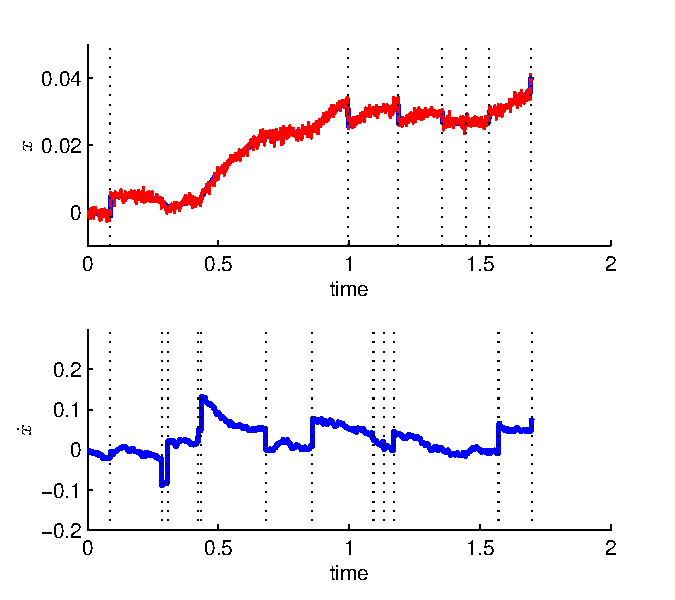
\includegraphics[width=0.9\columnwidth]{example_data.pdf}
\caption{An example simulated data set, showing value (top) and trend (bottom). Value observations are overlayed. Jump times are shown as dotted vertical lines.}
\label{fig:example_data}
\end{figure}

\begin{figure}[!t]
\centering
\subfloat[]{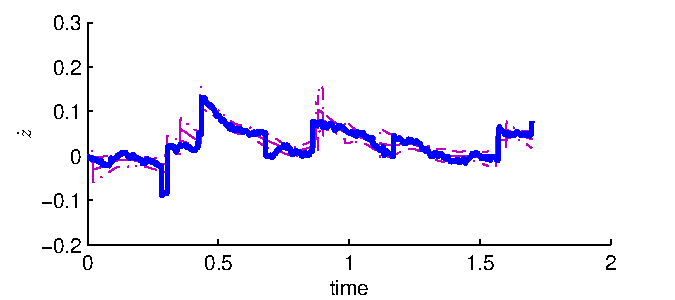
\includegraphics[width=0.9\columnwidth]{example_filtersmoother_state.pdf}} \\
\subfloat[]{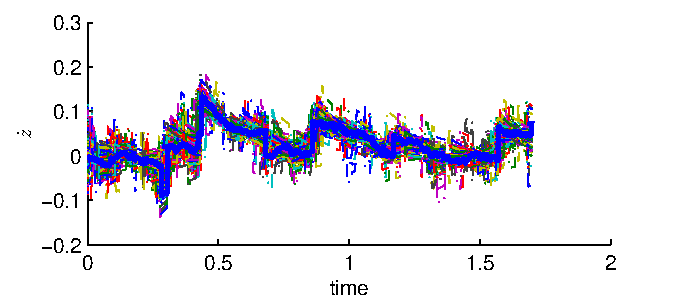
\includegraphics[width=0.9\columnwidth]{example_smoother_state.pdf}}
\caption{Trend estimates from (a) the filter-smoother and (b) the VRPS. Solid lines show means of each particle. Dashed lines show mean $\pm$2 standard deviations.}
\label{fig:example_state}
\end{figure}

Performance was evaluated by testing on 10 scenarios, each with 1000 observations. At each observation time, an estimate of the value and trend is made by taking the average of Gaussian means generated by an RTS smoother for each particle. The resulting root mean square errors (RMSEs) are displayed in table~\ref{tab:finance_state_performance}, demonstrating an improvement in accuracy from the smoother.

\begin{table}%
\caption{State estimation performance.}
\label{tab:finance_state_performance}
\centering
\renewcommand{\arraystretch}{1.5}
\begin{tabular}{|c|c|c|c|}
\hline
 &\raisebox{0cm}[0.4cm][0.3cm]{\parbox[c]{1.5cm}{\centering VRPF}} & \raisebox{0cm}[0.4cm][0.3cm]{\parbox[c]{1.5cm}{\centering Filter-smoother}} & \raisebox{0cm}[0.4cm][0.3cm]{\parbox[c]{1.5cm}{\centering VRPS}} \\
\hline \hline
\raisebox{0cm}[0.4cm][0.3cm]{\parbox[c]{2cm}{\centering mean value estimate RMSE}}   & $5.31 \times 10^{-4}$ & $4.48 \times 10^{-4}$ & $4.16 \times 10^{-4}$ \\
\hline
\raisebox{0cm}[0.4cm][0.3cm]{\parbox[c]{2cm}{\centering mean trend estimate RMSE}}   & $2.56 \times 10^{-2}$ & $1.79 \times 10^{-2}$ & $1.49 \times 10^{-2}$ \\
\hline
\end{tabular}
\end{table}

The mean number of unique particle estimates at each time step is shown in Fig.~\ref{fig:finance_unique_particles}. This illustrates the main advantage of the smoother algorithm --- the increased number of unique particles in the approximation means a better characterisation of the posterior changepoint and state distributions.

\begin{figure}[!t]
\centering
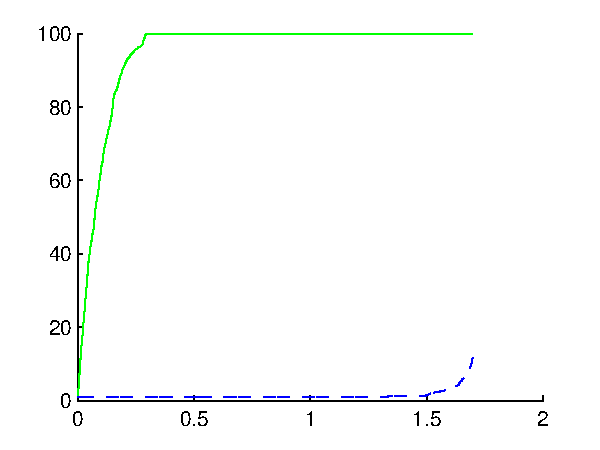
\includegraphics[width=0.75\columnwidth]{finance_unique_particles.pdf}
\caption{Mean number of unique particles in the filter-smoother (dashed) and smoother (solid) estimates.}
\label{fig:finance_unique_particles}
\end{figure}



\subsection{Conditionally Deterministic Model}

The piecewise-deterministic variable rate algorithms were tested on the intrinsic coordinate tracking model outlined in section~\ref{sec:tracking_model} using artificial simulated data. The changepoint motion parameters are assumed to be independent and zero-mean Gaussian distributed. The times between changepoints are modelled as gamma distributed. Observations are made via a radar-style bearing and range measurement model with Gaussian noise.

The filtering and smoothing algorithms were tested on artificial data simulated from the model. Observations were generated every $0.1s$. The variances of tangential and normal accelerations were set to $0.01m/s^2$ and $1m/s^2$ respectively, and those for the drift velocities to $1m/s$. The parameters of the Gamma distribution for inter-changepoint times were $5$ and $1s$ for the shape and scale respectively. Observation noise standard deviations were $0.1m$ and $0.25^{\circ}$ respectively.

The filter and smoother were each used to generate $50$ particles, with the filter employing resample-move steps with proposals based on an unscented transform \cite{Julier2004} approximation to the optimal proposal density.

An example trajectory is shown in Fig.~\ref{fig:simulated_trajectory}, with the results of the VRPF and VRPS algorithms in Fig.\ref{fig:2D_particle_results}. The improved particle diversity achieved by the smoothing algorithm is readily apparent.

\begin{figure}[!t]
\centering
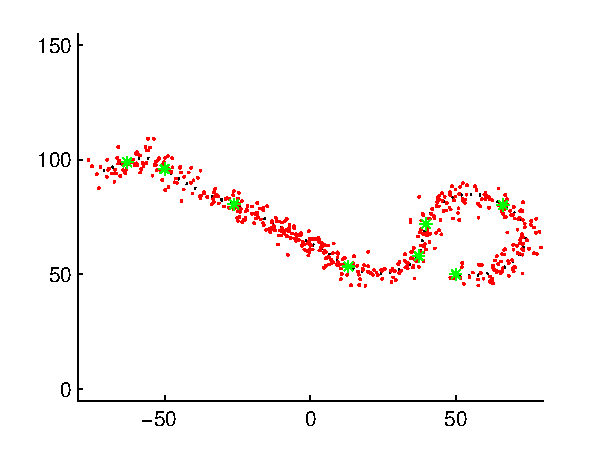
\includegraphics[width=0.9\columnwidth]{simulated_problem.pdf}
\caption{An example simulated data set, showing true position (dashed line), observations (dots) and changepoint positions (crosses). }
\label{fig:simulated_trajectory}
\end{figure}

\begin{figure}[!t]
\centering
\subfloat[]{\includegraphics[width=0.9\columnwidth]{2DFilter.pdf}} \\
\subfloat[]{\includegraphics[width=0.9\columnwidth]{2DSmoother.pdf}}
\caption{Filter (a) and smoother (b) particle estimates of position (solid lines), with particle changepoint positions (crosses). }
\label{fig:2D_particle_results}
\end{figure}

Performance was evaluated by testing on 10 independently generated scenarios, each with 500 observations. At each observation time, an estimate of the position and velocity is made by taking the average of values from the array of particles. The resulting root mean square errors (RMSEs) are displayed in table~\ref{tab:tracking_state_performance}, demonstrating an improvement in accuracy from the smoother. The VRPS also provides a more accurate estimate of the number of changepoints in each test, with an average error of 0.6 compared to 2.0 from the filter-smoother.

The mean number of unique particle estimates at each time step is shown in Fig.~\ref{fig:tracking_unique_particles}. This illustrates again the principal advantage of the VRPS algorithm --- the increased number of unique particles in the approximation means a better characterisation of the posterior changepoint distribution, allowing, for example, calculation of state covariances.

\begin{table}%
\caption{State estimation performance.}
\label{tab:tracking_state_performance}
\centering
\renewcommand{\arraystretch}{1.5}
\begin{tabular}{|c|c|c|c|}
\hline
 &\raisebox{0cm}[0.4cm][0.3cm]{\parbox[c]{1.5cm}{\centering VRPF}} & \raisebox{0cm}[0.4cm][0.3cm]{\parbox[c]{1.5cm}{\centering Filter-smoother}} & \raisebox{0cm}[0.4cm][0.3cm]{\parbox[c]{1.5cm}{\centering VRPS}} \\
% & \begin{minipage}[c]{1.5cm}\centering RBVRPF + KF\end{minipage} & \begin{minipage}[c]{1.5cm}\centering RBVRPF + RTS\end{minipage} & \begin{minipage}[c]{1.5cm}\centering RBVRPS + RTS\end{minipage} \\
\hline \hline
\raisebox{0cm}[0.4cm][0.3cm]{\parbox[c]{2cm}{\centering mean position estimate RMSE}} & 2.14 & 1.36 & 1.12 \\
\hline
\raisebox{0cm}[0.4cm][0.3cm]{\parbox[c]{2cm}{\centering mean velocity estimate RMSE}} & 1.89 & 1.03 & 0.85 \\
\hline
\end{tabular}
\end{table}

\begin{figure}[!t]
\centering
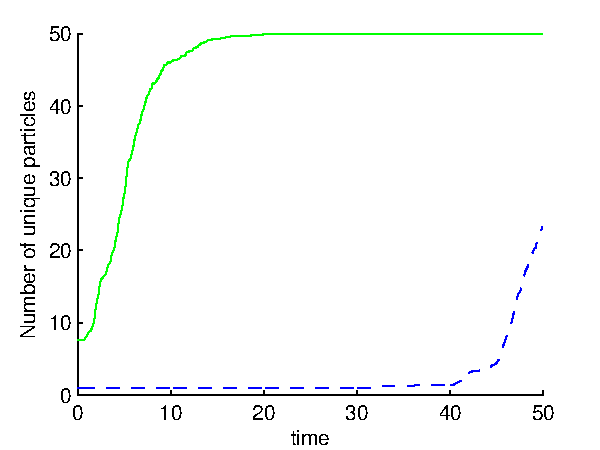
\includegraphics[width=0.75\columnwidth]{tracking_unique_particles.pdf}
\caption{Mean number of unique particles in the final filter (dashed) and smoother (solid) estimates.}
\label{fig:tracking_unique_particles}
\end{figure}



\section{Conclusions}

New smoothing algorithms have been introduced for variable rate models which have either linear-Gaussian or deterministic dynamics conditional on a set of unknown changepoints. For the linear-Gaussian case, the algorithm employs Rao-Blackwellisation, using particle methods to estimate the nonlinear changepoint sequence, and Kalman filtering/smoothing to estimate the linear state components. For the deterministic case, smoothing is achieved by sampling an augmented target distribution using MCMC. Simulations demonstrate that the smoothers generate approximations with improved particle diversity and accuracy when compared to the filters.



\appendices
\section{The Backwards Kalman Filter} \label{app:backwards_KF}

A backwards Kalman filter \cite{Fraser1969,Kitagawa1994} is used to calculate the joint likelihood term, $p(y_{n+1:N}|x_n, \tilde{\theta}_{n}^+)$, when the state dynamics are linear-Gaussian. Assume that at time $t_{n+1}$ there is a Gaussian density such that,
%
\begin{equation}
 p(y_{n+1:N}|x_{n+1}, \tilde{\theta}_{n}^+) = \tilde{Z}_{n+1} \mathcal{N}(x_{n+1}|\tilde{m}_{n+1}, \tilde{P}_{n+1}) \nonumber    .
\end{equation}

The state transition model is linear-Gaussian, so the backwards predictive density is given by,
%
\begin{IEEEeqnarray}{rCl}
\IEEEeqnarraymulticol{3}{l}{p(y_{n+1:N}|x_n, \tilde{\theta}_{n}^+)} \nonumber \\
  & = & \int p(y_{n+1:N}|x_{n+1}, \tilde{\theta}_{n}^+)  p(x_{n+1}|x_n, \tilde{\theta}_{n}^+) dx_{n+1} \nonumber \\
  & = & \int \tilde{Z}_{n+1} \mathcal{N}(x_{n+1}|\tilde{m}_{n+1}, \tilde{P}_{n+1}) \nonumber \\
  &   & \qquad \mathcal{N}(x_{n+1}|A_{n+1} x_{n}, Q_{n+1}) dx_{n+1} \nonumber \\
  & = & \int \tilde{Z}_{n+1} ||A_{n+1}^{-1}|| \mathcal{N}(x_{n+1}|\tilde{m}_{n+1}, \tilde{P}_{n+1}) \nonumber \\
  &   & \qquad \mathcal{N}(x_{n}|A_{n+1}^{-1} x_{n+1}, A_{n+1}^{-1} Q_{n+1} A_{n+1}^{-T}) dx_{n+1} \nonumber \\
  & = & \tilde{Z}_{n}^- \mathcal{N}(x_n|\tilde{m}_n^-, \tilde{P}_n^-) \nonumber
\end{IEEEeqnarray}

where,
%
\begin{IEEEeqnarray}{rCl}
 \tilde{m}_n^- & = & A_{n+1}^{-1} \tilde{m}_{n+1} \nonumber \\
 \tilde{P}_n^- & = & A_{n+1}^{-1} (\tilde{P}_{n+1} + Q_{n+1}) A_{n+1}^{-T} \nonumber \\
 \tilde{Z}_n^- & = & \tilde{Z}_{n+1} ||A_{n+1}||^{-1} \nonumber   .
\end{IEEEeqnarray}

$||A||$ denotes the magnitude of the determinant of $A$, and it is assumed that $A$ is non-singular.

The update step simply involves multiplying by the likelihood of the observation at time $t_n$,
%
\begin{IEEEeqnarray}{rCl}
\IEEEeqnarraymulticol{3}{l}{p(y_{n:N}|x_n, \tilde{\theta}_{n}^+)} \nonumber \\
 & = & p(y_{n+1:N}|x_n, \tilde{\theta}_{n}^+) p(y_{n}|x_n, \tilde{\theta}_{n}^+) \nonumber \\
 & = & \tilde{Z}_n^- \mathcal{N}(x_n|\tilde{m}_n^-, \tilde{P}_n^-) \mathcal{N}(y_n|C_n x_n, R_n) \nonumber \\
 & = & \tilde{Z}_n \mathcal{N}(x_n|\tilde{m}_n, \tilde{P}_n) \nonumber     ,
\end{IEEEeqnarray}

where,
%
\begin{IEEEeqnarray}{rCl}
 \tilde{\mu}_n & = & C_n \tilde{m}_n^-  \nonumber \\
 \tilde{S}_n   & = & C_n \tilde{P}_n^- C_n^T + R_n  \nonumber \\
 \tilde{G}_n   & = & \tilde{P}_n^- C_n^T \tilde{S}_n^{-1} \nonumber \\
 \tilde{m}_n   & = & \tilde{m}_n^- + \tilde{G}_n (y_n - \tilde{\mu}_n) \nonumber \\
 \tilde{P}_n   & = & \tilde{P}_n^- - \tilde{G}_n \tilde{S}_n \tilde{G}_n^T \nonumber \\
 \tilde{Z}_n   & = & \tilde{Z}_n^- \mathcal{N}(y_n|\tilde{\mu}_n, \tilde{S}_n) \nonumber   .
\end{IEEEeqnarray}

All steps use only standard Gaussian identities.



\section{Initialisation of the Backwards Kalman Filter} \label{app:init_backwards_KF}

The backwards Kalman filter recursion may be initialised exactly by inversion of the observation model using the method of \cite{Kitagawa1994}. By stacking up the last $L+1$ observations into a single vector, it is possible to write down a joint Gaussian distribution conditional on the $(N-L)$th state. This may be inverted to produce an improper Gaussian density for $x_{N-L}$,
%
\begin{IEEEeqnarray}{rCl}
 \IEEEeqnarraymulticol{3}{l}{p(y_{N-L:N}|x_{N-L}) = \mathcal{N}( \mathbf{y}_{N-L:N} | H_{N-L} x_{N-L}, \Gamma_{N-L} ) } \nonumber \\
 & = & \sqrt{\frac{|V_{N-L}|}{|\Gamma_{N-L}|}} \mathcal{N}(x_{N-L} | \nu_{N-L}, V_{N-L} ) \nonumber
\end{IEEEeqnarray}
\begin{IEEEeqnarray}{rCl}
 V_{N-L} & = & (H_{N-L}^T \Gamma_{N-L}^{-1} H_{N-L})^{-1} \nonumber \\
 \nu_{N-L} & = & V_{N-L} H_{N-L}^T \Gamma_{N-L}^{-1} \mathbf{y}_{N-L:N} \nonumber     ,
\end{IEEEeqnarray}

where $\mathbf{y}_{N-L:N}$ is a vector of concatenated observations, and $H_{N-L}$ and $\Gamma_{N-L}$ may be constructed from the system models,
%
\begin{IEEEeqnarray}{rCl}
\mathbf{y}_{N-L:N} & = & \begin{bmatrix}y_N \\ y_{N-1} \\ \vdots \\ y_{N-L} \end{bmatrix} \nonumber \\
%\end{IEEEeqnarray}
%\begin{IEEEeqnarray}{rCl}
H_{N-L} & = & \begin{bmatrix} C A^L \\ C A^{L-1} \\ \vdots \\ C \end{bmatrix} \nonumber \\
%\end{IEEEeqnarray}
%\begin{IEEEeqnarray}{rCl}
 \Gamma_{N-1} & = & K_{N-L} \begin{bmatrix} Q_N & 0 & \dots & 0 \\ 0 & Q_{N-1} & \dots & 0 \\ \vdots & \vdots & \ddots & \vdots \\ 0 & 0 & \dots & Q_{N-L+1} \end{bmatrix} K_{N-L}^T \nonumber \\
  & & + \: \begin{bmatrix} R_N & 0 & \dots & 0 \\ 0 & R_{N-1} & \dots & 0 \\ \vdots & \vdots & \ddots & \vdots \\ 0 & 0 & \dots & R_{N-L} \end{bmatrix} \nonumber \\
%\end{IEEEeqnarray}
%\begin{IEEEeqnarray}{rCl}
 K_{N-L} & = & \begin{bmatrix} C & CA & \dots & CA^{L-1} \\ 0 & C & \dots & CA^{L-2} \\ \vdots & \vdots & \ddots & \vdots \\ 0 & 0 & \dots & C \\ 0 & 0 & \dots & 0 \end{bmatrix} \nonumber
\end{IEEEeqnarray}

In the above, it is assumed for clarity that $A_n = A$ and $C_n = C$ are constant matrices. This assumption is easily relaxed. This inversion should be effected for the smallest value of $L$ such that the matrix inverses exist.






\section{Discretisation of the Jump-Diffusion Model} \label{app:lg_model_discretisation}

State evolution is governed by the following stochastic differential equation,
%
\begin{IEEEeqnarray}{c}
 dx(t) = \begin{bmatrix}0 & 1 \\ 0 & -\lambda \end{bmatrix} x(t) dt + \begin{bmatrix}0 \\ \sigma \end{bmatrix} d\beta(t) + dJ(t) \nonumber
\end{IEEEeqnarray}

where $\lambda$ is the mean reversion constant, $\sigma$ is the diffusion constant, $\beta(t)$ is standard Brownian motion, $dJ(t)$ is a jump term defined according to,
%
\begin{IEEEeqnarray}{rCl}
 dJ(t) & = & \begin{cases} J_k & t \in \{\tau_k\} \\ 0 & \text{elsewhere} \end{cases} \nonumber \\
 J_k  & \sim & \mathcal{N}(J_k| 0, Q_{J,u_k}) \nonumber    .
\end{IEEEeqnarray}

$\{\tau_k\}$ is the set of jump times, and $\{u_k\}$ the set of jump types, where $u_k = 1$ indicates a value jump, and $u_k=2$ a trend jump. The jump covariance matrices are,
%
\begin{IEEEeqnarray}{c}
Q_{J,u_k} = \begin{cases} \begin{bmatrix}\sigma_{J1}^2 & 0 \\ 0 & 0 \end{bmatrix} & u_k = 1 \\
                          \begin{bmatrix}0 & 0 \\ 0 & \sigma_{J2}^2 \end{bmatrix} & u_k = 2  \end{cases} \nonumber    .
\end{IEEEeqnarray}

Discretisation proceeds by separating the diffusion and jump terms and integrating separately. The jump term is straightforward to integrate. The diffusion term is a standard linear time invariant stochastic differential equation, and may be solved using the methods described in, for example, \cite{Oksendal2003,Grewal2002}. Matrix fraction decomposition is used for solving the covariance propagation equation \cite{Grewal2002,Sarkka2006}. The resulting discrete-time system is governed by a difference equation,
%
\begin{IEEEeqnarray}{rCl}
 x_n &=& A x_{n-1} + w_n \nonumber
\end{IEEEeqnarray}

where the $w_n$ is a Gaussian random variable with covariance matrix $Q_n$. The inter-observation time is denoted $\Delta t = t_{n} - t_{n-1}$, and,
%
\begin{IEEEeqnarray}{rCl}
 A     &=& \begin{bmatrix}1 & \frac{1}{\lambda}(1-e^{(-\lambda \Delta t)} \\ 0 & e^{(-\lambda \Delta t)}\end{bmatrix} \nonumber \\
 Q_n   &=& \begin{cases}Q_{D} + Q_{J,u_k} & \exists k : \tau_k \in [t_{n-1},t_n]\\
                        Q_{D}             & \text{otherwise} \end{cases} \nonumber \\
 Q_{D} &=& \frac{\sigma^2}{2 \lambda}\begin{bmatrix} q_1 & q_2 \\ q_2 & q_3\end{bmatrix} \nonumber \\
 q_1   &=& \frac{1}{\lambda^2}(2 \lambda \Delta t - (3 - e^{(-\lambda \Delta t)})(1 - e^{(-\lambda \Delta t)})~) \nonumber \\
 q_2   &=& \frac{1}{\lambda} (1-e^{(-\lambda \Delta t)})^2 \nonumber \\
 q_3   &=& 1-e^{(-2 \lambda \Delta t)} \nonumber     .
\end{IEEEeqnarray}

Assuming only the value is observed, corrupted by Gaussian noise with standard deviation $\sigma_y^2$, the measurement model is defined by,
%
\begin{IEEEeqnarray}{rCl}
 y_n &=& C x_{n} + v_n \nonumber
\end{IEEEeqnarray}

where $v_n$ is a Gaussian random variable with covariance matrix $R$.
%
\begin{IEEEeqnarray}{rCl}
 C &=& \begin{bmatrix}1 & 0\end{bmatrix} \nonumber \\
 R &=& \sigma_y^2  \nonumber    .
\end{IEEEeqnarray}



%\newpage
\bibliographystyle{IEEEtran}
\bibliography{D:/pb404/Dropbox/PhD/Cleanbib}

%\begin{IEEEbiography}[{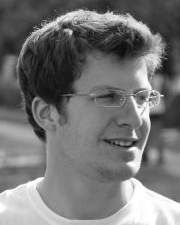
\includegraphics[width=1in,height=1.25in,clip,keepaspectratio]{D:/pb404/Dropbox/PhD/Biographies/Bunch-bw.jpg}}]{Pete Bunch} (M'11) has an MEng. degree from the University of Cambridge, UK, and is currently cogitating towards a PhD degree in signal processing at the Cambridge University Engineering Department.

He is an enthusiastic Bayesian, with research interests in sequential inference, numerical approximations and target tracking.
\end{IEEEbiography}
%\begin{IEEEbiography}[{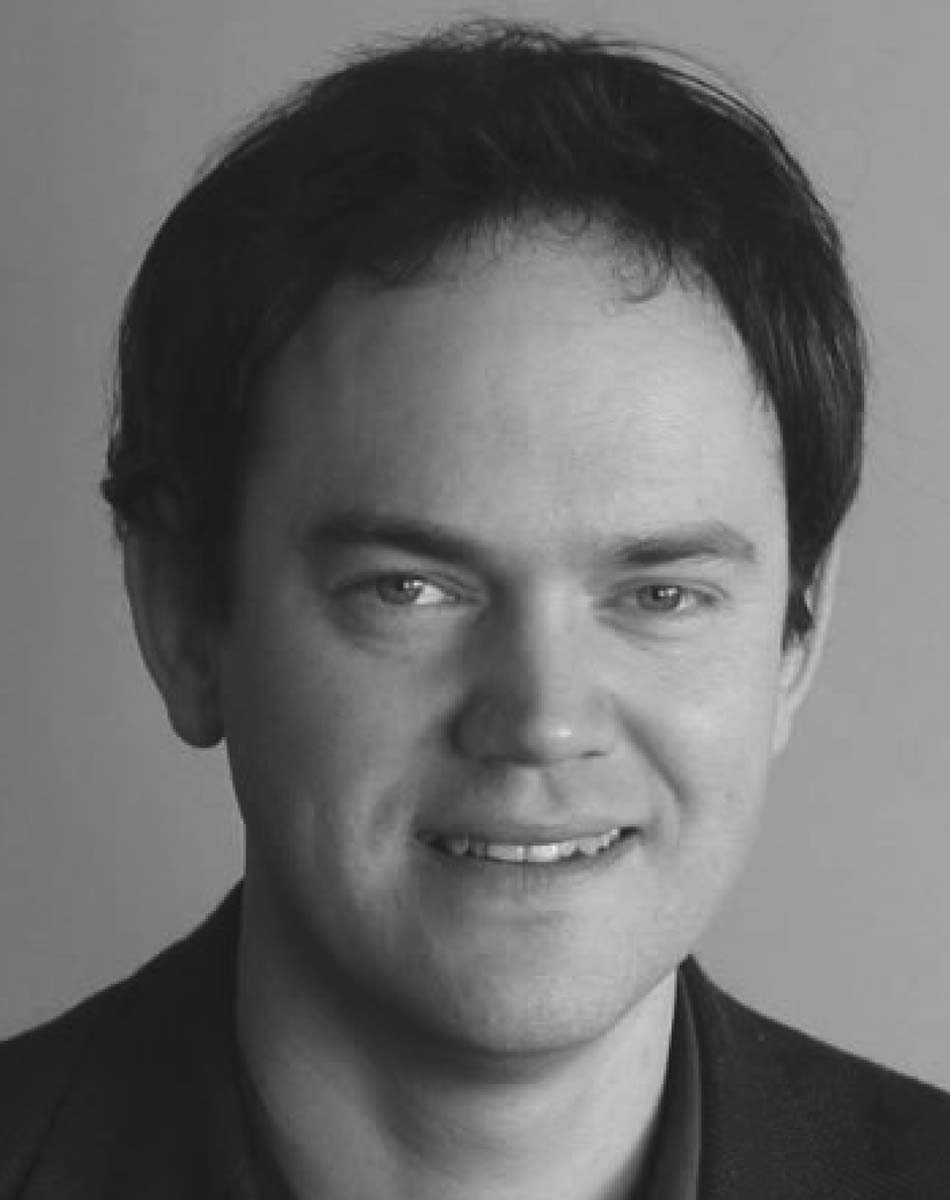
\includegraphics[width=1in,height=1.25in,clip,keepaspectratio]{Godsill.jpg}}]{Simon Godsill} is Professor of Statistical Signal Processing in the Engineering Department at Cambridge University and a Professorial Fellow and tutor at Corpus Christi College Cambridge.

He coordinates an active research group in Signal Inference and its Applications within the Signal Processing and Communications Laboratory at Cambridge, specialising in Bayesian computational methodology, multiple object tracking, audio and music processing, and financial time series modeling. A particular methodological theme over recent years has been the development of novel techniques  for optimal Bayesian filtering and smoothing, using Sequential Monte Carlo or Particle Filtering methods.

Prof. Godsill has published extensively in journals, books and international conference proceedings. He was technical chair of the IEEE NSSPW workshop in 2006 on sequential and nonlinear filtering methods, was Technical Chair for Fusion 2010 in Edinburgh, and has been on the conference panel for numerous other conferences and workshops. Prof. Godsill has served as Associate Editor for IEEE Tr. Signal Processing and the journal Bayesian Analysis. He was Theme Leader in Tracking and Reasoning over Time for the UK�s Data and Information Fusion Defence Technology Centre (DIF-DTC) and Principal Investigator on grants funded by the EU, EPSRC, QinetiQ, General Dynamics, MOD, Microsoft UK, Citibank and Mastercard. In 2009-10 he was co-organiser of an 18 month research program in Sequential Monte Carlo Methods at the SAMSI Institute in North Carolina. He is a Director of CEDAR Audio Ltd. (which has received a technical Oscar for its audio processing work), and Input Dynamics Ltd., both companies which use his research work in the audio area.   


\end{IEEEbiography} 

\end{document}
%%%%%%%%%%%%%%%%%%%%%%%%%%%%%%%%%%%%%%%%%%%%%%%%%%%%%%%%%%%%%%%%%%%%%%%%%%%%%%%%%%%%%%%%%%%%%%%%%%%%%%%%%%%%%%%%%%%%


























